\documentclass[a4paper,14pt]{extarticle}
\usepackage{../../tex-shared/report-layout}

\renewcommand{\mylabnumber}{3}
\renewcommand{\mylabtitle}{Исследование процессов моделирования данных, информационного
                           моделирования процессов и построение реляционных информационных
                           структур при помощи методологий ERD, IDEF1, IDEF1X с
                           использованием CASE-средств}
\renewcommand{\mysubject}{Методы и средства проектирования информационных систем}
\renewcommand{\mylecturer}{Заикина Е.Н.}

\begin{document}
\begin{titlepage}
    
    \thispagestyle{empty}
    
    \begin{center}
        
        Министерство науки и Высшего образования Российской Федерации \\
        Севастопольский государственный университет \\
        Кафедра ИС
        
        \vfill

        Отчет \\
        по лабораторной работе №\mylabnumber \\
        \enquote{\mylabtitle} \\
        по дисциплине \\
        \enquote{\MakeTextUppercase{\mysubject}}

    \end{center}

    \vspace{1cm}

    \noindent\hspace{7.5cm} Выполнил студент группы ИС/б-17-2-о \\
    \null\hspace{7.5cm} Горбенко К. Н. \\
    \null\hspace{7.5cm} Проверил \\
    \null\hspace{7.5cm} \mylecturer

    \vfill

    \begin{center}
        Севастополь \\
        \the\year{}
    \end{center}

\end{titlepage}

\section{Цель работы}
Осуществить исследование и построение информационной модели в нотациях П. Чена и
IDEF1 (IDEF1X). Осуществить выбор и применение инструментального средства
информационного моделирования процессов и построения реляционных информационных
структур (IDEF1X диаграмм).

\section{Задание на работу}
В соответствии с вариантом предметной области и на основании результатов
выполнения лабораторных работ №1 и №2 выполнить построение IDEF1X-диаграммы при
помощи CASE-средства CA ERwin Data Modeler Community \\Edition.

\section{Ход работы}
\subsection{Описание предметной области}
Список потенциальных сущностей:

\begin{itemize}
    \item \textbf{Группа словарей.} Содержит информацию о группе словарей.
          Словари делятся на группы для классификации.
    \item \textbf{Словарь.} Содержит информацию о словаре. Используется для
          хранения переводов.
    \item \textbf{Перевод.} Содержит перевод: переводимое слово (выражение,
          предложение), его выбранные переводы, флеш-карточку (контекстную
          информацию).
    \item \textbf{Единица перевода.} Содержит одну единицу перевода (на родном
          языке) для того, чтобы переводы могли содержать список таких единиц.
    \item \textbf{Выбранный перевод.} Содержит связь между сущностями
          \enquote{Единица перевода} и \enquote{Перевод}.
    \item \textbf{Пользователь.} Содержит информацию о пользователе системы.
    \item \textbf{Тип упражнения.} Содержит все возможные типы упражнений.
    \item \textbf{Упражнение.} Содержит информацию о том, какое упражнение
          пользователь выполняет (выполнил), список вариантов ответа и 
    \item \textbf{Ответ пользователя при упражнении.} Содержит информацию об
          ответе пользователя при прохождении упражнения по переводу.
    \item \textbf{Экспорт группы словарей.} Содержит информацию о том, какому
          пользователю был предоставлен доступ к каким словарям или группам
          словарей.
\end{itemize}

Атрибуты сущностей:

\begin{itemize}
    \item \textbf{Группа словарей.} Id, дата удаления, Id пользователя, название, описание.
    \item \textbf{Словарь.} Id, дата удаления, Id группы словарей, название, описание.
    \item \textbf{Перевод.} Id, дата удаления, Id словаря, переводимое выражение, пользовательский контекс использования.
    \item \textbf{Единица перевода.} Id, название единицы перевода.
    \item \textbf{Выбранные перевод.} Id перевода, Id единицы перевода.
    \item \textbf{Пользователь.} Id, дата удаления, логин, пароль, электронная почта.
    \item \textbf{Тип упражнения.} Id, название типа упражнения.
    \item \textbf{Упражнение.} Id, Id типа упражнения, Id перевода, Id пользователя.
    \item \textbf{Ответ на упражнение.} Id, Id упражнения, Id единицы перевода, признак правильности выбора.
    \item \textbf{Экспорт группы словарей.} Id пользователя, Id группы словарей.
\end{itemize}

Описание предметной области на естественном языке:

\begin{enumerate}
    \item Каждая \textbf{группа словарей} может содержать несколько \textbf{словарей}.
    \item Каждый \textbf{словарь} может содержать несколько \textbf{переводов}.
    \item Каждый \textbf{перевод} может содержать несколько \textbf{выбранных переводов}.
    \item Каждый \textbf{выбранный перевод} относится только к одной \textbf{единице перевода}.
    \item Каждый \textbf{пользоваель} имеет несколько \textbf{групп словарей}.
    \item Каждое \textbf{упражнение} относится только к одному \textbf{типу упражнений}.
    \item Каждый \textbf{ответ на упражнение} является ответом только на одно \textbf{упражнение}.
    \item Каждый \textbf{экспорт группы словарей} относится только к одному пользователю.
    \item Каждый \textbf{экспорт группы словарей} относится только к одной группе словарей.
\end{enumerate}

Матрица отношений между сущностями:

\begin{landscape}
\begin{table}[H]
    \footnotesize
    \caption{Матрица отношений между сущностями}
    \begin{tabular}{ | p{1.9cm} | p{1.9cm} | p{1.9cm} | p{1.9cm} | p{1.9cm} | p{1.9cm} | p{1.9cm} | p{1.9cm} | p{1.9cm} | p{1.9cm} | p{1.9cm} | }
        \hline
        -- & Группа словарей & Словарь & Перевод & Выбранный перевод & Единица перевода  & Пользователь & Тип упражнения & Упражнение & Ответ на упражнение & Экспорт \\ \hline
        Группа словарей & -- & содержит (1:N) & & & & содержится (1:1) & & & & относится (1:1) \\ \hline
        Словарь & относится (1:1) & -- & содержит (1:N) & & & & & & & \\ \hline
        Перевод & & относится (1:1) & -- & содержит (1:N) & & & & содержит (1:N) & & \\ \hline
        Выбранный перевод & & & относится (1:1) & -- & относится (1:1) & & & & & \\ \hline
        Единица перевода & & & относится (1:1) & относится (1:1) & -- & & & & содержит (1:1) & \\ \hline
        Пользователь & содержит (1:N) & & & & & -- & & содержит (1:N) & & относится (1:1) \\ \hline
        Тип упражнения & & & & & & & -- & включает (1:N) & & \\ \hline
        Упражнение & & & относится (1:1) & & & & является (1:1) & -- & относится (1:1) & \\ \hline
        Ответ на упражнение & & & & & относится (1:1) & & & относится (1:1) & -- & \\ \hline
        Экспорт & относится (1:1) & & & & & относится (1:1) & & & & -- \\ \hline
    \end{tabular}
\end{table}
\pagebreak
\end{landscape}

\subsection{Составление диаграммы в нотации IDEF1X}
Составленная диаграмма в нотации IDEF1X представлена на рисунке
\ref{fig:idef1x}:

\begin{figure}[H]
    \centering
    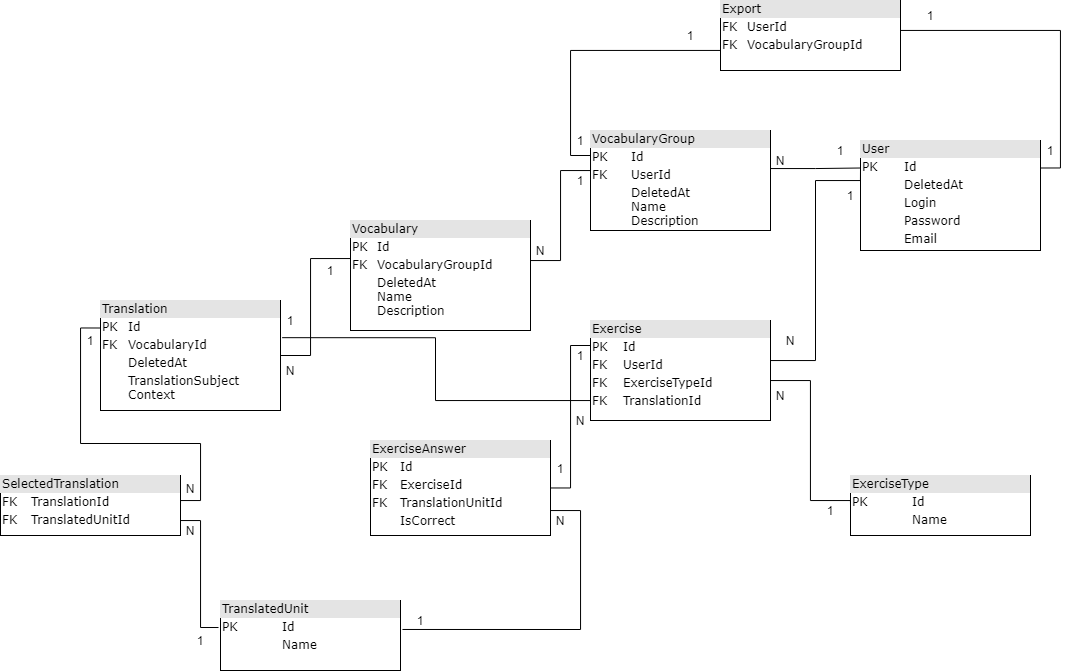
\includegraphics[width=\linewidth]{idef1x}
    \caption{Диаграмма предметной области в нотации IDEF1X}
    \label{fig:idef1x}
\end{figure}

\section*{Выводы}
В ходе выполнение лабораторной работы была освоена методология построения
информационной модели в нотации IDEF1X.
\end{document}